\chapter{状态值与贝尔曼方程}
\label{ch:rl-bellman}

% ════════════════════════════════════════════════════════════════
%  来源：赵世钰《强化学习的数学原理》第 2 章（源页 p037–p056，逐页核对）。
%  原原本本忠实转写：保留全部正文 / 公式 / 推导 / 表 / 示例 / 图注。
%  插图分层：图 2.1（本章在全书中的位置导航图）弃用，留 %TODO；
%  网格世界 / 状态转移示意（图 2.2/2.3/2.4/2.5/2.6/2.8）TikZ 重绘；
%  数据密集的策略-状态值网格阵列（图 2.7）用 \includegraphics。
% ════════════════════════════════════════════════════════════════

% TODO: 图 2.1「本章在全书中的位置」(Zhao 导航图) 弃用，不收录。
%       源 MD: images/64a6709ca45e8f9f9f72fb7f1a6e3d113671e2c8a0f432036fa470425e29786d.jpg

本章介绍一个核心概念和一个核心工具。抓住这两个核心就能很好地掌握本章的内容。这个核心概念是状态值，它很重要是因为它可以作为评价一个策略好坏的指标。既然状态值这么重要，那么我们怎么分析它呢？答案就是使用一个核心工具：贝尔曼方程。贝尔曼方程描述了所有状态值之间的关系：通过求解贝尔曼方程，我们就可以得到状态值，进而评价一个策略的好坏。

% ════════════════════════════════════════════════════════════════
\section{启发示例 1：为什么回报很重要？}
\label{sec:rl-bellman-why-return}

回报这个概念已经在第 1 章介绍过了，它在强化学习中扮演着重要的角色，这是因为它可以用来评价一个策略的好坏。我们通过下面的例子来说明这一点。\cref{fig:rl-bellman-three-policies} 给出了三个策略：这三个策略在状态 $s_1$ 是不同的，在其他状态是相同的。那么这三个策略哪一个是最好的、哪一个是最差的呢？

\begin{figure}[ht]
\centering
\begin{tikzpicture}[scale=0.85, >=Stealth,
  cell/.style={draw, minimum size=11mm, inner sep=0pt},
  forb/.style={cell, fill=second!22},
  targ/.style={cell, fill=third!20},
  arr/.style={->, thick, main!70!black}]
% 三个 2x2 网格，左右排列，间距大
\foreach \ox/\lab in {0/(a), 4/(b), 8/(c)}{
  % 画 2x2 单元格
  \node[forb] (b\ox) at (\ox+1,0.55) {};        % 右上 = 禁止区
  \node[cell] (a\ox) at (\ox+0,0.55) {$s_1$};   % 左上 = s1
  \node[cell] (c\ox) at (\ox+0,-0.55) {$s_3$};  % 左下 = s3
  \node[targ] (d\ox) at (\ox+1,-0.55) {$s_4$};  % 右下 = 目标区
  \node at (b\ox) {$s_2$};
}
% (a) s1 向下 r=0；s2 向下 r=1；s3 向右 r=1；s4 自环 r=1
\draw[arr] (a0.south) -- node[right, font=\tiny] {$r{=}0$} (c0.north);
\draw[arr] (b0.south) -- node[right, font=\tiny] {$r{=}1$} (d0.north);
\draw[arr] (c0.east) -- node[below, font=\tiny] {$r{=}1$} (d0.west);
\node[font=\tiny] at (1.55,-0.9) {$r{=}1$};
\node at (0.5,-1.5) {(a)};
% (b) s1 向右 r=-1；s2 向下 r=1；s3 向右 r=1；s4 自环 r=1
\draw[arr] (a4.east) -- node[above, font=\tiny] {$r{=}-1$} (b4.west);
\draw[arr] (b4.south) -- node[right, font=\tiny] {$r{=}1$} (d4.north);
\draw[arr] (c4.east) -- node[below, font=\tiny] {$r{=}1$} (d4.west);
\node[font=\tiny] at (5.55,-0.9) {$r{=}1$};
\node at (4.5,-1.5) {(b)};
% (c) s1 各 0.5：右 p=0.5 r=-1，下 p=0.5 r=0；s2 向下 r=1；s3 向右 r=1；s4 自环 r=1
\draw[arr] (a8.south) -- node[left, font=\tiny] {$p{=}0.5$} (c8.north);
\draw[arr] (a8.east) -- node[above, font=\tiny] {$p{=}0.5$} (b8.west);
\draw[arr] (b8.south) -- node[right, font=\tiny] {$r{=}1$} (d8.north);
\draw[arr] (c8.east) -- node[below, font=\tiny] {$r{=}1$} (d8.west);
\node[font=\tiny] at (9.55,-0.9) {$r{=}1$};
\node at (8.5,-1.5) {(c)};
\end{tikzpicture}
\caption{用于说明回报重要性的三个例子。这三个例子中的策略在 $s_1$ 中是不同的。}
\label{fig:rl-bellman-three-policies}
\end{figure}

这三个策略的好坏在直观上是很容易判断的：最左边的策略是最好的，因为从 $s_1$ 出发会避开禁止区域；中间的策略最差，因为从 $s_1$ 出发会进入禁止区域；最右边的策略相比前面两个既不好也不坏，因为它有 $0.5$ 的概率避开禁止区域，也有 $0.5$ 的概率进入禁止区域。

上面的直观判断能否用数学来描述呢？答案是可以的，这就依赖于“回报”这个概念。具体来说，假设智能体的初始状态是 $s_1$。

如果按照最左边的策略，得到的轨迹是 $s_1 \to s_3 \to s_4 \to s_4 \cdots$，相应的折扣回报是
\begin{equation*}
\begin{aligned}
\mathrm{return}_1 &= 0 + \gamma 1 + \gamma^2 1 + \dots \\
&= \gamma (1 + \gamma + \gamma^2 + \dots) \\
&= \frac{\gamma}{1 - \gamma},
\end{aligned}
\end{equation*}
其中 $\gamma \in (0,1)$ 是折扣因子。

如果按照中间的策略，得到的轨迹是 $s_1 \to s_2 \to s_4 \to s_4 \cdots$，相应的折扣回报是
\begin{equation*}
\begin{aligned}
\mathrm{return}_2 &= -1 + \gamma 1 + \gamma^2 1 + \dots \\
&= -1 + \gamma (1 + \gamma + \gamma^2 + \dots) \\
&= -1 + \frac{\gamma}{1 - \gamma}.
\end{aligned}
\end{equation*}

如果按照最右边的策略，可能得到两条轨迹：一条是 $s_1 \to s_3 \to s_4 \to s_4 \cdots$，另一条是 $s_1 \to s_2 \to s_4 \to s_4 \cdots$。这两条轨迹发生的概率都是 $0.5$。那么从 $s_1$ 开始可以获得的平均回报是
\begin{equation*}
\begin{aligned}
\mathrm{return}_3 &= 0.5 \left(-1 + \frac{\gamma}{1 - \gamma}\right) + 0.5 \left(\frac{\gamma}{1 - \gamma}\right) \\
&= -0.5 + \frac{\gamma}{1 - \gamma}.
\end{aligned}
\end{equation*}

通过比较上面计算出来的三个策略的回报，我们知道
\begin{equation}
\mathrm{return}_1 > \mathrm{return}_3 > \mathrm{return}_2
\label{eq:rl-bellman-return-order}
\end{equation}
这个不等式表明：第一个策略是最好的，因为它的回报最大；第二个策略是最差的，因为它的回报最小。这个数学结论与前面的直观判断是一致的：第一个策略是最好的，因为它可以避免进入禁止区域；而第二个策略是最差的，因为它会进入禁止区域。

上面的例子说明了一个重要结论：回报可以用来评价策略的好坏。不过值得注意的是，这里的 $\mathrm{return}_3$ 并没有严格遵守回报的定义：回报的定义只是针对一条轨迹，而 $\mathrm{return}_3$ 是两条轨迹回报的平均值。稍后我们就会知道 $\mathrm{return}_3$ 实际上就是本章要介绍的状态值。

% ════════════════════════════════════════════════════════════════
\section{启发示例 2：如何计算回报？}
\label{sec:rl-bellman-compute-return}

上一节展示了回报的重要性。既然回报这么重要，那么如何计算回报呢？有的读者可能会疑惑：回报可以基于它的定义来计算，为什么还要问这个问题？实际上，有两种计算回报的方法。

\medskip
$\diamond$ 第一种计算回报的方法就是根据其定义：回报等于沿轨迹收集的所有奖励的折扣总和。这种方法我们已经比较熟悉了。下面以 \cref{fig:rl-bellman-return-cycle} 为例再次介绍。令 $v_i$ 表示从 $s_i$ 开始得到的回报，其中 $i=1,2,3,4$。那么从这些状态出发得到的回报是
\begin{equation}
\begin{aligned}
& v_1 = r_1 + \gamma r_2 + \gamma^2 r_3 + \dots , \\
& v_2 = r_2 + \gamma r_3 + \gamma^2 r_4 + \dots , \\
& v_3 = r_3 + \gamma r_4 + \gamma^2 r_1 + \dots , \\
& v_4 = r_4 + \gamma r_1 + \gamma^2 r_2 + \dots .
\end{aligned}
\label{eq:rl-bellman-return-def}
\end{equation}

\begin{figure}[ht]
\centering
\begin{tikzpicture}[>=Stealth, scale=1.0,
  cell/.style={draw, minimum size=12mm, inner sep=0pt},
  arr/.style={->, thick, main!70!black}]
\node[cell] (s1) at (0,1.3) {$s_1$};
\node[cell] (s2) at (1.3,1.3) {$s_2$};
\node[cell] (s4) at (0,0) {$s_4$};
\node[cell] (s3) at (1.3,0) {$s_3$};
\draw[arr] (s1.east) -- node[above, font=\footnotesize] {$r_1$} (s2.west);
\draw[arr] (s2.south) -- node[right, font=\footnotesize] {$r_2$} (s3.north);
\draw[arr] (s3.west) -- node[below, font=\footnotesize] {$r_3$} (s4.east);
\draw[arr] (s4.north) -- node[left, font=\footnotesize] {$r_4$} (s1.south);
\end{tikzpicture}
\caption{用于说明如何计算回报的例子。简单起见，这个例子不含目标区域和禁止区域。}
\label{fig:rl-bellman-return-cycle}
\end{figure}

第二种方法是本节重点关注的自举法（bootstrapping）。具体来说，通过观察方程 \cref{eq:rl-bellman-return-def} 中回报的表达式，可以将它们重写为
\begin{equation}
\begin{aligned}
v_1 &= r_1 + \gamma (r_2 + \gamma r_3 + \ldots) = r_1 + \gamma v_2, \\
v_2 &= r_2 + \gamma (r_3 + \gamma r_4 + \ldots) = r_2 + \gamma v_3, \\
v_3 &= r_3 + \gamma (r_4 + \gamma r_1 + \ldots) = r_3 + \gamma v_4, \\
v_4 &= r_4 + \gamma (r_1 + \gamma r_2 + \ldots) = r_4 + \gamma v_1.
\end{aligned}
\label{eq:rl-bellman-bootstrap}
\end{equation}

方程 \cref{eq:rl-bellman-bootstrap} 展示了一个有趣的现象：从不同状态出发的回报值是彼此依赖的。具体来说，$v_1$ 依赖于 $v_2$，$v_2$ 依赖于 $v_3$，$v_3$ 依赖于 $v_4$，而 $v_4$ 又依赖于 $v_1$。这反映了自举的思想：$v_1,v_2,v_3,v_4$ 可以从其自身 $v_2,v_3,v_4,v_1$ 得到。

乍一看，自举是一个无解的循环，这是因为一个未知量的计算依赖于另一个未知量。但是如果从数学的角度来看，自举则非常容易理解。具体来说，方程 \cref{eq:rl-bellman-bootstrap} 可以被重新整理成一个矩阵-向量形式的线性方程：
\begin{equation}
\underbrace{\begin{bmatrix} v_1 \\ v_2 \\ v_3 \\ v_4 \end{bmatrix}}_{v \in \mathbb{R}^4}
= \begin{bmatrix} r_1 \\ r_2 \\ r_3 \\ r_4 \end{bmatrix}
+ \begin{bmatrix} \gamma v_2 \\ \gamma v_3 \\ \gamma v_4 \\ \gamma v_1 \end{bmatrix}
= \underbrace{\begin{bmatrix} r_1 \\ r_2 \\ r_3 \\ r_4 \end{bmatrix}}_{r \in \mathbb{R}^4}
+ \gamma \underbrace{\begin{bmatrix}
0 & 1 & 0 & 0 \\
0 & 0 & 1 & 0 \\
0 & 0 & 0 & 1 \\
1 & 0 & 0 & 0
\end{bmatrix}}_{P \in \mathbb{R}^{4 \times 4}}
\underbrace{\begin{bmatrix} v_1 \\ v_2 \\ v_3 \\ v_4 \end{bmatrix}}_{v \in \mathbb{R}^4},
\label{eq:rl-bellman-toy-matrix}
\end{equation}
上式可以简化为
\begin{equation*}
v = r + \gamma P v.
\end{equation*}

如果大家学过线性代数，相信不难求解出上面方程的解：$v = (I - \gamma P)^{-1} r$，其中 $I \in \mathbb{R}^{4 \times 4}$ 是单位矩阵。有的读者可能会问 $(I - \gamma P)$ 一定是可逆的吗？答案是肯定的，具体证明会在 \cref{sec:rl-bellman-analytic} 中给出。

事实上，方程 \cref{eq:rl-bellman-bootstrap} 就是这个简单例子对应的贝尔曼方程，而方程 \cref{eq:rl-bellman-toy-matrix} 是这个贝尔曼方程的矩阵-向量形式。尽管很简单，但方程 \cref{eq:rl-bellman-bootstrap} 展示了贝尔曼方程的核心思想：从一个状态出发获得的回报依赖于从其他状态出发时获得的回报。这个思想对于理解后面介绍的贝尔曼方程至关重要。

% ════════════════════════════════════════════════════════════════
\section{状态值}
\label{sec:rl-bellman-state-value}

虽然前面提到了回报可以用来评价策略，但是回报并不适用于一般化的随机情况，因为从一个状态出发可能会得到不同的轨迹和回报。为此，我们需要引入状态值的概念。

首先，我们需要引入一些符号。在时刻 $t = 0,1,2,\ldots$，智能体处于状态 $S_t$，按照策略 $\pi$ 采取动作 $A_t$，转移到的下一个状态是 $S_{t+1}$，获得的即时奖励是 $R_{t+1}$。这个过程可以简洁地表达为
\begin{equation*}
S_t \xrightarrow{A_t} S_{t+1}, R_{t+1}.
\end{equation*}
这里 $S_t, S_{t+1} \in \mathcal{S}$，$A_t \in \mathcal{A}(S_t)$，$R_{t+1} \in \mathcal{R}(S_t, A_t)$。请注意，这里 $S_t, S_{t+1}, A_t, R_{t+1}$ 都是随机变量（random variables）。本书一般用大写字母表示随机变量。

从时刻 $t$ 开始，我们可以得到一条包含一系列“状态-动作-奖励”的轨迹：
\begin{equation*}
S_t \xrightarrow{A_t} S_{t+1}, R_{t+1} \xrightarrow{A_{t+1}} S_{t+2}, R_{t+2} \xrightarrow{A_{t+2}} S_{t+3}, R_{t+3}, \ldots
\end{equation*}
根据定义，沿这个轨迹得到的折扣回报是
\begin{equation*}
G_t \doteq R_{t+1} + \gamma R_{t+2} + \gamma^2 R_{t+3} + \dots ,
\end{equation*}
其中 $\gamma \in (0,1)$ 是折扣因子。请注意，$G_t$ 也是一个随机变量，因为它是 $R_{t+1}, R_{t+2}, \ldots$ 这些随机变量组合得到的。

由于 $G_t$ 是一个随机变量，因此我们可以计算它的期望值（expectation 或 expected value）为
\begin{equation}
v_\pi(s) \doteq \mathbb{E}[G_t \mid S_t = s].
\label{eq:rl-bellman-state-value-def}
\end{equation}
这里 $v_\pi(s)$ 称为状态值函数（state-value function）。一般简称为状态值或状态价值（state value）。下面是对状态值的一些说明。

\medskip
$\diamond$ 第一，$v_\pi(s)$ 的值依赖于 $s$，即不同状态的状态值一般是不同的。这是因为 $v_\pi(s)$ 在 \cref{eq:rl-bellman-state-value-def} 中的定义是一个条件期望，而其中的条件是 $S_t = s$。关于条件期望的介绍可以参见附录 A。

\medskip
$\diamond$ 第二，$v_\pi(s)$ 的值依赖于 $\pi$，即不同策略对应的状态值一般是不同的。这是因为轨迹是根据策略 $\pi$ 得到的，不同的策略可能导致不同的轨迹。

\medskip
$\diamond$ 第三，$v_\pi(s)$ 并不依赖于 $t$。虽然 $v_\pi(s)$ 在 \cref{eq:rl-bellman-state-value-def} 中的定义涉及时刻 $t$，但是不论 $t$ 选取什么值得到的结果都是相同的，这本质上是因为系统是平稳的，不会随着时间变化。

“状态值”与“回报”是什么关系呢？当策略和系统模型都是确定性时，从一个状态出发始终会得到相同的轨迹。此时，从一个状态出发得到的回报就等于状态值。相反，当策略或系统模型是随机的时，从一个状态出发可能产生不同的轨迹。此时，不同轨迹的回报是不同的，而状态值就是这些回报的期望值。因此，状态值比回报更加一般化，能够同时处理确定性和随机性的情况。因此，虽然我们在 \cref{sec:rl-bellman-why-return} 提到回报可以用来评价策略，但是更一般化地应该用状态值来评价策略：能产生更高状态值的策略更好。

正因为状态值能够用于评价策略，所以它是强化学习中的一个核心概念。既然状态值这么重要，那么该如何计算状态值呢？这个问题将在下一节回答。

% ════════════════════════════════════════════════════════════════
\section{贝尔曼方程}
\label{sec:rl-bellman-equation}

本节将介绍大名鼎鼎的贝尔曼方程（Bellman equation），它是用于分析状态值的核心工具。用一句话概述：贝尔曼方程描述了所有状态值之间的关系。

下面我们详细推导贝尔曼方程。首先，$G_t$ 可以重写为
\begin{equation*}
\begin{aligned}
G_t &= R_{t+1} + \gamma R_{t+2} + \gamma^2 R_{t+3} + \dots \\
&= R_{t+1} + \gamma (R_{t+2} + \gamma R_{t+3} + \dots) \\
&= R_{t+1} + \gamma G_{t+1},
\end{aligned}
\end{equation*}
其中 $G_{t+1} = R_{t+2} + \gamma R_{t+3} + \ldots$。该方程建立了 $G_t$ 和 $G_{t+1}$ 之间的关系。因此，状态值可以写成
\begin{equation}
\begin{aligned}
v_\pi(s) &= \mathbb{E}[G_t \mid S_t = s] \\
&= \mathbb{E}[R_{t+1} + \gamma G_{t+1} \mid S_t = s] \\
&= \mathbb{E}[R_{t+1} \mid S_t = s] + \gamma \mathbb{E}[G_{t+1} \mid S_t = s].
\end{aligned}
\label{eq:rl-bellman-split}
\end{equation}
下面我们分别分析式 \cref{eq:rl-bellman-split} 中的两项。

\medskip
$\diamond$ 第一项 $\mathbb{E}[R_{t+1} \mid S_t = s]$ 是即时奖励的期望值。基于全期望（total expectation）的性质（参见附录 A），这一项可以化为
\begin{equation}
\begin{aligned}
\mathbb{E}[R_{t+1} \mid S_t = s] &= \sum_{a \in \mathcal{A}} \pi(a \mid s) \, \mathbb{E}[R_{t+1} \mid S_t = s, A_t = a] \\
&= \sum_{a \in \mathcal{A}} \pi(a \mid s) \sum_{r \in \mathcal{R}} p(r \mid s, a) \, r.
\end{aligned}
\label{eq:rl-bellman-immediate}
\end{equation}
这里 $\mathcal{A}$ 和 $\mathcal{R}$ 分别是可能的动作和可能的奖励的集合。对于不同的状态，$\mathcal{A}$ 可能是不同的；此时 $\mathcal{A}$ 可以表示为 $\mathcal{A}(s)$。类似地，$\mathcal{R}$ 也可能依赖于 $(s, a)$。

\medskip
$\diamond$ 第二项 $\mathbb{E}[G_{t+1} \mid S_t = s]$ 是未来奖励的期望值。它可以计算为
\begin{equation}
\begin{aligned}
\mathbb{E}[G_{t+1} \mid S_t = s] &= \sum_{s' \in \mathcal{S}} \mathbb{E}[G_{t+1} \mid S_t = s, S_{t+1} = s'] \, p(s' \mid s) \\
&= \sum_{s' \in \mathcal{S}} \mathbb{E}[G_{t+1} \mid S_{t+1} = s'] \, p(s' \mid s) \qquad (\text{由于马尔可夫性质}) \\
&= \sum_{s' \in \mathcal{S}} v_\pi(s') \, p(s' \mid s) \\
&= \sum_{s' \in \mathcal{S}} v_\pi(s') \sum_{a \in \mathcal{A}} p(s' \mid s, a) \, \pi(a \mid s).
\end{aligned}
\label{eq:rl-bellman-future}
\end{equation}
上述推导过程中使用了 $\mathbb{E}[G_{t+1} \mid S_t = s, S_{t+1} = s'] = \mathbb{E}[G_{t+1} \mid S_{t+1} = s']$ 的结果，该结果成立是由于马尔可夫性质，即未来的奖励仅依赖于当前状态，而与先前的状态无关。

将式 \cref{eq:rl-bellman-immediate}～\cref{eq:rl-bellman-future} 代入式 \cref{eq:rl-bellman-split} 可得
\begin{equation}
\begin{aligned}
v_\pi(s) &= \mathbb{E}[R_{t+1} \mid S_t = s] + \gamma \mathbb{E}[G_{t+1} \mid S_t = s] \\
&= \underbrace{\sum_{a \in \mathcal{A}} \pi(a \mid s) \sum_{r \in \mathcal{R}} p(r \mid s, a) \, r}_{\text{即时奖励的期望}}
+ \underbrace{\gamma \sum_{a \in \mathcal{A}} \pi(a \mid s) \sum_{s' \in \mathcal{S}} p(s' \mid s, a) \, v_\pi(s')}_{\text{未来奖励的期望}} \\
&= \sum_{a \in \mathcal{A}} \pi(a \mid s) \left[ \sum_{r \in \mathcal{R}} p(r \mid s, a) \, r + \gamma \sum_{s' \in \mathcal{S}} p(s' \mid s, a) \, v_\pi(s') \right], \quad s \in \mathcal{S}.
\end{aligned}
\label{eq:rl-bellman-main}
\end{equation}
上式就是大名鼎鼎的贝尔曼方程，它描述了不同状态值之间的关系，是设计和分析强化学习算法的基本工具。

贝尔曼方程乍一看似乎很复杂，但实际上它的结构非常清晰。下面是对该方程的解释说明。

\medskip
$\diamond$ $v_\pi(s)$ 和 $v_\pi(s')$ 是需要计算的状态值，是未知量。如果单独看式 \cref{eq:rl-bellman-main}，因为状态值存在于等式的两边，读者可能难以理解如何求解。必须要注意的是，每一个状态 $s \in \mathcal{S}$ 都对应了式 \cref{eq:rl-bellman-main}，所以我们有一组这样的式子。如果我们将这些式子联立，如何计算所有状态值就变得很清晰了。详细内容将在 \cref{sec:rl-bellman-solve} 中给出。

\medskip
$\diamond$ $\pi(a \mid s)$ 是一个给定的策略，是已知量。贝尔曼方程一定是对应了一个特定的策略。求解贝尔曼方程从而得到状态值是一个策略评价（policy evaluation）的过程，这是许多强化学习算法中的核心步骤。

\medskip
$\diamond$ $p(r \mid s, a)$ 和 $p(s' \mid s, a)$ 代表系统模型，这是已知量还是未知量呢？在本书中，我们将首先研究模型已知的情况，例如在 \cref{sec:rl-bellman-solve} 给出模型已知情况下如何计算状态值。在本书后面的章节中，我们会慢慢推广到不需要模型的情况。

除了式 \cref{eq:rl-bellman-main} 中的表达式外，读者在文献中还可能见到过贝尔曼方程的其他表达形式。接下来我们介绍三种常见的等价形式。

\medskip
$\diamond$ 第一个等价形式是
\begin{equation*}
v_\pi(s) = \sum_{a \in \mathcal{A}} \pi(a \mid s) \sum_{s' \in \mathcal{S}} \sum_{r \in \mathcal{R}} p(s', r \mid s, a) \left[ r + \gamma v_\pi(s') \right].
\end{equation*}
这实际上是文献 [3] 使用的表达式。这个式子可以通过将下面的全概率公式（参见附录 A）代入式 \cref{eq:rl-bellman-main} 得到：
\begin{equation*}
\begin{aligned}
p(s' \mid s, a) &= \sum_{r \in \mathcal{R}} p(s', r \mid s, a), \\
p(r \mid s, a) &= \sum_{s' \in \mathcal{S}} p(s', r \mid s, a).
\end{aligned}
\end{equation*}

\medskip
$\diamond$ 第二个常见的等价形式是贝尔曼期望方程（Bellman expectation equation）：
\begin{equation*}
v_\pi(s) = \mathbb{E}\big[ R_{t+1} + \gamma v_\pi(S_{t+1}) \mid S_t = s \big], \quad s \in \mathcal{S}.
\end{equation*}
这是因为 $\mathbb{E}[G_{t+1} \mid S_t = s] = \sum_a \pi(a \mid s) \sum_{s'} p(s' \mid s, a) v_\pi(s') = \mathbb{E}[v_\pi(S_{t+1}) \mid S_t = s]$，将其代入 \cref{eq:rl-bellman-split} 即可得到贝尔曼期望方程。

\medskip
$\diamond$ 第三，奖励 $r$ 在某些问题中可能仅依赖于下一个状态 $s'$，即奖励可以写成 $r(s')$。此时我们有 $p(r(s') \mid s, a) = p(s' \mid s, a)$，将其代入 \cref{eq:rl-bellman-main} 可得另外一个表达式
\begin{equation*}
v_\pi(s) = \sum_{a \in \mathcal{A}} \pi(a \mid s) \sum_{s' \in \mathcal{S}} p(s' \mid s, a) \left[ r(s') + \gamma v_\pi(s') \right].
\end{equation*}

% ════════════════════════════════════════════════════════════════
\section{示例}
\label{sec:rl-bellman-examples}

本节将使用两个例子来演示如何得到贝尔曼方程进而求解状态值。建议读者仔细阅读这些例子，它们能很好地帮助大家理解贝尔曼方程。

\begin{example}[确定性策略]
\label{ex:rl-bellman-deterministic}
\cref{fig:rl-bellman-ex-deterministic} 给出了一个确定性的策略。我们下面一步一步地写出贝尔曼方程，然后求解状态值。

首先，考虑状态 $s_1$，其对应的策略是 $\pi(a = a_3 \mid s_1) = 1$ 和 $\pi(a \neq a_3 \mid s_1) = 0$；对应的状态转移概率为 $p(s' = s_3 \mid s_1, a_3) = 1$ 和 $p(s' \neq s_3 \mid s_1, a_3) = 0$；对应的奖励概率为 $p(r = 0 \mid s_1, a_3) = 1$ 和 $p(r \neq 0 \mid s_1, a_3) = 0$。将这些概率代入 \cref{eq:rl-bellman-main} 可以得到
\begin{equation}
v_\pi(s_1) = 0 + \gamma v_\pi(s_3).
\label{eq:rl-bellman-ex1-s1}
\end{equation}
有趣的是，虽然 \cref{eq:rl-bellman-main} 中贝尔曼方程的表达式看起来很复杂，但是 \cref{eq:rl-bellman-ex1-s1} 却非常简单。式 \cref{eq:rl-bellman-main} 之所以那么复杂是为了能够描述所有一般情况。

\begin{figure}[H]
\centering
\begin{tikzpicture}[>=Stealth, scale=1.0,
  cell/.style={draw, minimum size=14mm, inner sep=0pt},
  forb/.style={cell, fill=second!22},
  targ/.style={cell, fill=third!20},
  arr/.style={->, thick, main!70!black}]
\node[cell] (s1) at (0,1.4) {$s_1$};
\node[forb] (s2) at (1.4,1.4) {};
\node at (s2) {$s_2$};
\node[cell] (s3) at (0,0) {$s_3$};
\node[targ] (s4) at (1.4,0) {$s_4$};
\node at (s4) {$s_4$};
\node[font=\footnotesize] at (-0.45,0.7) {$r=0$};
\draw[arr] (s1.south) -- (s3.north);
\draw[arr] (s2.south) -- node[right, font=\footnotesize] {$r=1$} (s4.north);
\draw[arr] (s3.east) -- node[below, font=\footnotesize] {$r=1$} (s4.west);
\node[font=\footnotesize] at (2.1,-0.5) {$r=1$};
\end{tikzpicture}
\caption{用于演示贝尔曼方程的例子。这个例子中的策略是确定性的。}
\label{fig:rl-bellman-ex-deterministic}
\end{figure}

由于这个例子非常简单，我们也可以直接根据贝尔曼方程的基本思想快速写出 \cref{eq:rl-bellman-ex1-s1}，而不用使用复杂的 \cref{eq:rl-bellman-main}。具体来说，从 $s_1$ 出发的回报（这里是 $v_\pi(s_1)$）等于即时奖励（这里是 $0$）加上从下一个状态出发的回报（这里是 $v_\pi(s_3)$），这样可以直接写出来 \cref{eq:rl-bellman-ex1-s1}。

类似的，对其他状态可以得到
\begin{equation*}
\begin{aligned}
& v_\pi(s_2) = 1 + \gamma v_\pi(s_4), \\
& v_\pi(s_3) = 1 + \gamma v_\pi(s_4), \\
& v_\pi(s_4) = 1 + \gamma v_\pi(s_4).
\end{aligned}
\end{equation*}
下一步我们可以从这些方程中解出状态值。由于这些方程非常简单，因此我们可以手动求解。更复杂的方程可以通过 \cref{sec:rl-bellman-solve} 中介绍的算法来求解。为简单起见，我们直接给出结果：
\begin{equation*}
\begin{aligned}
& v_\pi(s_4) = \frac{1}{1 - \gamma}, \\
& v_\pi(s_3) = \frac{1}{1 - \gamma}, \\
& v_\pi(s_2) = \frac{1}{1 - \gamma}, \\
& v_\pi(s_1) = \frac{\gamma}{1 - \gamma}.
\end{aligned}
\end{equation*}
进一步将 $\gamma = 0.9$ 代入上式可得
\begin{align*}
v_\pi(s_4) &= \frac{1}{1 - 0.9} = 10, \\
v_\pi(s_3) &= \frac{1}{1 - 0.9} = 10, \\
v_\pi(s_2) &= \frac{1}{1 - 0.9} = 10, \\
v_\pi(s_1) &= \frac{0.9}{1 - 0.9} = 9.
\end{align*}
\end{example}

\begin{example}[随机策略]
\label{ex:rl-bellman-stochastic}
\cref{fig:rl-bellman-ex-stochastic} 中的策略稍微复杂了一些，因为它是随机的。接下来，我们写出贝尔曼方程，然后从中求解状态值。

\begin{figure}[H]
\centering
\begin{tikzpicture}[>=Stealth, scale=1.0,
  cell/.style={draw, minimum size=14mm, inner sep=0pt},
  forb/.style={cell, fill=second!22},
  targ/.style={cell, fill=third!20},
  arr/.style={->, thick, main!70!black}]
\node[cell] (s1) at (0,1.4) {$s_1$};
\node[forb] (s2) at (1.4,1.4) {};
\node at (s2) {$s_2$};
\node[cell] (s3) at (0,0) {$s_3$};
\node[targ] (s4) at (1.4,0) {$s_4$};
\node at (s4) {$s_4$};
\node[font=\footnotesize, align=left] at (-0.05,2.25) {$p=0.5$\\ $r=-1$};
\node[font=\footnotesize, align=left] at (-0.6,0.55) {$r=0$\\ $p=0.5$};
\draw[arr] (s1.south) -- (s3.north);
\draw[arr] (s1.east) -- (s2.west);
\draw[arr] (s2.south) -- node[right, font=\footnotesize] {$r=1$} (s4.north);
\draw[arr] (s3.east) -- node[below, font=\footnotesize] {$r=1$} (s4.west);
\node[font=\footnotesize] at (2.1,-0.5) {$r=1$};
\end{tikzpicture}
\caption{用于演示贝尔曼方程的例子。这个例子中的策略是随机的。}
\label{fig:rl-bellman-ex-stochastic}
\end{figure}

首先，在状态 $s_1$，策略向右或向下移动的概率都是 $0.5$，即 $\pi(a = a_2 \mid s_1) = 0.5$ 和 $\pi(a = a_3 \mid s_1) = 0.5$；状态转移概率是 $p(s' = s_3 \mid s_1, a_3) = 1$ 和 $p(s' = s_2 \mid s_1, a_2) = 1$；奖励的概率是 $p(r = 0 \mid s_1, a_3) = 1$ 和 $p(r = -1 \mid s_1, a_2) = 1$。将这些概率值代入 \cref{eq:rl-bellman-main} 可得
\begin{equation*}
v_\pi(s_1) = 0.5 [0 + \gamma v_\pi(s_3)] + 0.5 [-1 + \gamma v_\pi(s_2)].
\end{equation*}
类似地，对其他状态可得
\begin{equation*}
\begin{aligned}
& v_\pi(s_2) = 1 + \gamma v_\pi(s_4), \\
& v_\pi(s_3) = 1 + \gamma v_\pi(s_4), \\
& v_\pi(s_4) = 1 + \gamma v_\pi(s_4).
\end{aligned}
\end{equation*}
状态值可以从上述方程中求解得到：
\begin{equation*}
\begin{aligned}
& v_\pi(s_4) = \frac{1}{1 - \gamma}, \\
& v_\pi(s_3) = \frac{1}{1 - \gamma}, \\
& v_\pi(s_2) = \frac{1}{1 - \gamma},
\end{aligned}
\end{equation*}
\begin{equation*}
\begin{aligned}
v_\pi(s_1) &= 0.5 [0 + \gamma v_\pi(s_3)] + 0.5 [-1 + \gamma v_\pi(s_2)] \\
&= -0.5 + \frac{\gamma}{1 - \gamma}.
\end{aligned}
\end{equation*}
进一步将 $\gamma = 0.9$ 代入上式可得
\begin{equation*}
\begin{aligned}
& v_\pi(s_4) = 10, \\
& v_\pi(s_3) = 10, \\
& v_\pi(s_2) = 10, \\
& v_\pi(s_1) = -0.5 + 9 = 8.5.
\end{aligned}
\end{equation*}
\end{example}

最后，如果我们比较上述例子中两个策略的状态值，可以看出
\begin{equation*}
v_{\pi_1}(s_i) \geqslant v_{\pi_2}(s_i), \quad i = 1, 2, 3, 4.
\end{equation*}
这说明 \cref{fig:rl-bellman-ex-deterministic} 中的策略更好，因为它具有更高的状态值。这个数学结论与直觉是一致的：直觉上第一种策略也是更好的，因为当智能体从 $s_1$ 出发时，它会避开禁止区域。因此，上述两个例子也说明了状态值可以用来评价策略的好坏。

% ════════════════════════════════════════════════════════════════
\section{矩阵-向量形式}
\label{sec:rl-bellman-matrix}

由于每一个状态都对应了式 \cref{eq:rl-bellman-main} 中的方程，因此我们可以联立所有这些方程进而得到简洁的矩阵-向量形式（matrix-vector form），该形式对理解和分析贝尔曼方程有重要作用。

为了推导出矩阵-向量形式，首先将式 \cref{eq:rl-bellman-main} 中的贝尔曼方程重写为
\begin{equation}
v_\pi(s) = r_\pi(s) + \gamma \sum_{s' \in \mathcal{S}} p_\pi(s' \mid s) \, v_\pi(s'),
\label{eq:rl-bellman-rewrite}
\end{equation}
其中
\begin{equation*}
\begin{aligned}
r_\pi(s) &\doteq \sum_{a \in \mathcal{A}} \pi(a \mid s) \sum_{r \in \mathcal{R}} p(r \mid s, a) \, r, \\
p_\pi(s' \mid s) &\doteq \sum_{a \in \mathcal{A}} \pi(a \mid s) \, p(s' \mid s, a).
\end{aligned}
\end{equation*}
这里 $r_\pi(s)$ 表示即时奖励的期望值，而 $p_\pi(s' \mid s)$ 代表在策略 $\pi$ 下从状态 $s$ 经过一步转移到状态 $s'$ 的概率。

为了写成矩阵-向量形式，需要对状态进行编号。如果有 $n = |\mathcal{S}|$ 个状态，那么给这 $n$ 个状态编号为 $\{s_1, s_2, \ldots, s_n\}$。对于状态 $s_i$，\cref{eq:rl-bellman-rewrite} 可以写成
\begin{equation}
v_\pi(s_i) = r_\pi(s_i) + \gamma \sum_{s_j \in \mathcal{S}} p_\pi(s_j \mid s_i) \, v_\pi(s_j).
\label{eq:rl-bellman-rewrite-i}
\end{equation}
定义 $v_\pi = [v_\pi(s_1), \dots, v_\pi(s_n)]^{\mathrm{T}} \in \mathbb{R}^n$，$r_\pi = [r_\pi(s_1), \dots, r_\pi(s_n)]^{\mathrm{T}} \in \mathbb{R}^n$，以及 $P_\pi \in \mathbb{R}^{n \times n}$，其中 $P_\pi$ 满足 $[P_\pi]_{ij} = p_\pi(s_j \mid s_i)$。此时 \cref{eq:rl-bellman-rewrite-i} 可以用下列矩阵-向量形式来表示：
\begin{equation}
v_\pi = r_\pi + \gamma P_\pi v_\pi,
\label{eq:rl-bellman-mv}
\end{equation}
这里 $v_\pi$ 是待解的未知量，而 $\gamma$、$r_\pi$、$P_\pi$ 是已知量。

矩阵 $P_\pi$ 有一些有趣的性质。第一，它是一个非负矩阵（non-negative matrix），即它所有元素都大于或等于 $0$。这个性质可以表示为 $P_\pi \geqslant 0$，其中 $0$ 表示具有适当维度的零矩阵。在本书中，“$\geqslant$”或“$\leqslant$”代表两个矩阵或者向量元素间的比较。第二，$P_\pi$ 是一个随机矩阵（stochastic matrix），即每一行所有元素之和等于 $1$。这个性质的数学表示为 $P_\pi \mathbf{1} = \mathbf{1}$，其中 $\mathbf{1} = [1, \ldots, 1]^{\mathrm{T}}$ 是一个具有合适维度的所有元素都是 $1$ 的向量。

\begin{figure}[ht]
\centering
\begin{tikzpicture}[>=Stealth, scale=1.0,
  cell/.style={draw, minimum size=14mm, inner sep=0pt},
  forb/.style={cell, fill=second!22},
  targ/.style={cell, fill=third!20},
  arr/.style={->, thick, main!70!black}]
\node[cell] (s1) at (0,1.4) {$s_1$};
\node[forb] (s2) at (1.4,1.4) {};
\node at (s2) {$s_2$};
\node[cell] (s3) at (0,0) {$s_3$};
\node[targ] (s4) at (1.4,0) {$s_4$};
\node at (s4) {$s_4$};
\node[font=\footnotesize, align=left] at (-0.05,2.25) {$p=0.5$\\ $r=-1$};
\node[font=\footnotesize, align=left] at (-0.6,0.55) {$r=0$\\ $p=0.5$};
\draw[arr] (s1.south) -- (s3.north);
\draw[arr] (s1.east) -- (s2.west);
\draw[arr] (s2.south) -- node[right, font=\footnotesize] {$r=1$} (s4.north);
\draw[arr] (s3.east) -- node[below, font=\footnotesize] {$r=1$} (s4.west);
\node[font=\footnotesize] at (2.1,-0.5) {$r=1$};
\end{tikzpicture}
\caption{用于说明贝尔曼方程矩阵-向量形式的例子。}
\label{fig:rl-bellman-mv-example}
\end{figure}

下面考虑 \cref{fig:rl-bellman-mv-example} 中给出的具体例子，其贝尔曼方程的矩阵-向量形式如下：
\begin{equation*}
\underbrace{\begin{bmatrix} v_\pi(s_1) \\ v_\pi(s_2) \\ v_\pi(s_3) \\ v_\pi(s_4) \end{bmatrix}}_{v_\pi}
= \underbrace{\begin{bmatrix} r_\pi(s_1) \\ r_\pi(s_2) \\ r_\pi(s_3) \\ r_\pi(s_4) \end{bmatrix}}_{r_\pi}
+ \gamma \underbrace{\begin{bmatrix}
p_\pi(s_1 \mid s_1) & p_\pi(s_2 \mid s_1) & p_\pi(s_3 \mid s_1) & p_\pi(s_4 \mid s_1) \\
p_\pi(s_1 \mid s_2) & p_\pi(s_2 \mid s_2) & p_\pi(s_3 \mid s_2) & p_\pi(s_4 \mid s_2) \\
p_\pi(s_1 \mid s_3) & p_\pi(s_2 \mid s_3) & p_\pi(s_3 \mid s_3) & p_\pi(s_4 \mid s_3) \\
p_\pi(s_1 \mid s_4) & p_\pi(s_2 \mid s_4) & p_\pi(s_3 \mid s_4) & p_\pi(s_4 \mid s_4)
\end{bmatrix}}_{P_\pi}
\underbrace{\begin{bmatrix} v_\pi(s_1) \\ v_\pi(s_2) \\ v_\pi(s_3) \\ v_\pi(s_4) \end{bmatrix}}_{v_\pi}.
\end{equation*}
将具体值代入上述方程式可得
\begin{equation*}
\begin{bmatrix} v_\pi(s_1) \\ v_\pi(s_2) \\ v_\pi(s_3) \\ v_\pi(s_4) \end{bmatrix}
= \begin{bmatrix} 0.5(0) + 0.5(-1) \\ 1 \\ 1 \\ 1 \end{bmatrix}
+ \gamma \begin{bmatrix}
0 & 0.5 & 0.5 & 0 \\
0 & 0 & 0 & 1 \\
0 & 0 & 0 & 1 \\
0 & 0 & 0 & 1
\end{bmatrix}
\begin{bmatrix} v_\pi(s_1) \\ v_\pi(s_2) \\ v_\pi(s_3) \\ v_\pi(s_4) \end{bmatrix}.
\end{equation*}
可以看出，$P_\pi$ 满足 $P_\pi \mathbf{1} = \mathbf{1}$。

% ════════════════════════════════════════════════════════════════
\section{求解状态值}
\label{sec:rl-bellman-solve}

给定一个策略，在得到其对应的贝尔曼方程后，我们可以从中求解出所有状态值。求解一个策略对应的状态值是强化学习中的一个基本问题，这个问题通常被称为策略评价。本节将给出两种求解贝尔曼方程的方法。

\subsection{方法 1：解析解}
\label{sec:rl-bellman-analytic}

由于 $v_\pi = r_\pi + \gamma P_\pi v_\pi$ 是一个简单的线性方程，我们不难得到其解析解：
\begin{equation}
v_\pi = (I - \gamma P_\pi)^{-1} r_\pi.
\label{eq:rl-bellman-closed-form}
\end{equation}
下面给出矩阵 $(I - \gamma P_\pi)^{-1}$ 的几个性质。

\medskip
$\diamond$ 第一，$I - \gamma P_\pi$ 是可逆的。证明如下。根据圆盘定理（Gershgorin circle theorem）[4]，$I - \gamma P_\pi$ 的每个特征值都至少位于一个 Gershgorin 圆盘内。具体来说，第 $i$ 个 Gershgorin 圆盘的中心位于 $[I - \gamma P_\pi]_{ii} = 1 - \gamma p_\pi(s_i \mid s_i)$，半径等于 $\sum_{j \neq i} \bigl| [I - \gamma P_\pi]_{ij} \bigr| = \sum_{j \neq i} \gamma p_\pi(s_j \mid s_i)$。因为 $\gamma < 1$，所以其半径小于该圆中心距离原点的距离：$\sum_{j \neq i} \gamma p_\pi(s_j \mid s_i) < 1 - \gamma p_\pi(s_i \mid s_i)$。因此，所有 Gershgorin 圆盘都不包含原点，进而可知 $I - \gamma P_\pi$ 没有等于 $0$ 的特征值。

\medskip
$\diamond$ 第二，$(I - \gamma P_\pi)^{-1} \geqslant I$，即矩阵 $(I - \gamma P_\pi)^{-1}$ 的每个元素都是大于或等于 $0$ 的，并且进一步来说是大于或等于单位矩阵 $I$ 中的相应元素。这是因为 $P_\pi$ 的元素是非负的，考虑矩阵逆的级数展开可得 $(I - \gamma P_\pi)^{-1} = I + \gamma P_\pi + \gamma^2 P_\pi^2 + \cdots \geqslant I \geqslant 0$。

\medskip
$\diamond$ 第三，对于任何向量 $r \geqslant 0$，有 $(I - \gamma P_\pi)^{-1} r \geqslant r \geqslant 0$。这个性质可由第二个性质推论得出，因为 $[(I - \gamma P_\pi)^{-1} - I] r \geqslant 0$。类似的，如果 $r_1 \geqslant r_2$，则有 $(I - \gamma P_\pi)^{-1} r_1 \geqslant (I - \gamma P_\pi)^{-1} r_2$。

\subsection{方法 2：数值解}
\label{sec:rl-bellman-numerical}

虽然解析解对于理论分析非常有用，但是因为它涉及矩阵逆运算，因此仍然需要复杂的数值算法来计算。实际上，我们可以直接使用如下数值迭代算法从贝尔曼方程中求解出状态值：
\begin{equation}
v_{k+1} = r_\pi + \gamma P_\pi v_k, \quad k = 0, 1, 2, \ldots
\label{eq:rl-bellman-iterative}
\end{equation}
从一个初始猜测 $v_0 \in \mathbb{R}^n$ 出发，该算法会给出一个序列 $\{v_0, v_1, v_2, \ldots\}$，并且该序列会逐渐收敛到真实的状态值，即
\begin{equation}
v_k \to v_\pi = (I - \gamma P_\pi)^{-1} r_\pi, \quad \text{随着} \ k \to \infty .
\label{eq:rl-bellman-converge}
\end{equation}
式 \cref{eq:rl-bellman-converge} 的证明在方框 2.1 中给出。

\begin{derivation}[方框 2.1：证明 \texorpdfstring{\cref{eq:rl-bellman-converge}}{(2.15)}]
定义误差为 $\delta_k = v_k - v_\pi$。我们只需要证明 $\delta_k \to 0$。将 $v_{k+1} = \delta_{k+1} + v_\pi$ 和 $v_k = \delta_k + v_\pi$ 代入 $v_{k+1} = r_\pi + \gamma P_\pi v_k$ 可得
\begin{equation*}
\delta_{k+1} + v_\pi = r_\pi + \gamma P_\pi (\delta_k + v_\pi).
\end{equation*}
上式可以变换为
\begin{equation*}
\begin{aligned}
\delta_{k+1} &= -v_\pi + r_\pi + \gamma P_\pi \delta_k + \gamma P_\pi v_\pi \\
&= \gamma P_\pi \delta_k - v_\pi + (r_\pi + \gamma P_\pi v_\pi) \\
&= \gamma P_\pi \delta_k.
\end{aligned}
\end{equation*}
由上式进一步可得
\begin{equation*}
\delta_{k+1} = \gamma P_\pi \delta_k = \gamma^2 P_\pi^2 \delta_{k-1} = \dots = \gamma^{k+1} P_\pi^{k+1} \delta_0.
\end{equation*}
由于 $P_\pi$ 的每个元素都大于或等于 $0$ 并且小于或等于 $1$，我们有 $0 \leqslant P_\pi^k \leqslant 1$ 对任何 $k$ 都成立。另一方面，因为 $\gamma < 1$，所以当 $k \to \infty$ 时有 $\gamma^k \to 0$。因此，当 $k \to \infty$ 时有 $\delta_{k+1} = \gamma^{k+1} P_\pi^{k+1} \delta_0 \to 0$。
\end{derivation}

\subsection{示例}
\label{sec:rl-bellman-solve-examples}

下面我们用前两个小节介绍的算法来求解一些例子的状态值。具体求解过程不再展示，这里重点关注求解得到的状态值具有什么样的规律。

\cref{fig:rl-bellman-policy-grid} 中橙色的单元格表示禁止区域，蓝色的单元格代表目标区域。奖励设置为 $r_{\mathrm{boundary}} = r_{\mathrm{forbidden}} = -1$，$r_{\mathrm{target}} = 1$。折扣因子选取为 $\gamma = 0.9$。

\cref{fig:rl-bellman-policy-grid}(a) 给出了两个“好”的策略及其对应的状态值。虽然这两个策略有相同的状态值，但是在第四列的前两个状态的策略是不同。因此，我们知道不同的策略可能拥有相同的状态值。

\cref{fig:rl-bellman-policy-grid}(b) 展示了两个“不好”的策略及其对应的状态值。这两个策略之所以不好，是因为许多状态对应的策略从直觉上就是不合理的。而这种直觉与我们计算得到的状态值是一致的，例如这两个策略的状态值都是负的，比 \cref{fig:rl-bellman-policy-grid}(a) 中“好”策略的状态值都要小。

\begin{figure}[H]
\centering
% (a) 两个“好”的策略：左策略图 + 右状态值表（两份，状态值相同）
\begin{minipage}{\linewidth}
\centering
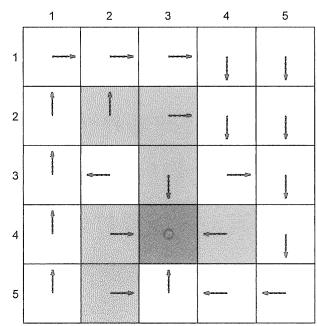
\includegraphics[width=0.32\linewidth]{figures/rl/53607a99fd24d5a72f24ef5718700386c7a3782c058a2ae9fb3c38c0509f4678}\hfill
\begin{minipage}{0.30\linewidth}\centering\footnotesize
\begin{tabular}{c|ccccc}
 & 1 & 2 & 3 & 4 & 5 \\ \hline
1 & 3.5 & 3.9 & 4.3 & 4.8 & 5.3 \\
2 & 3.1 & 3.5 & 4.8 & 5.3 & 5.9 \\
3 & 2.8 & 2.5 & 10.0 & 5.9 & 6.6 \\
4 & 2.5 & 10.0 & 10.0 & 10.0 & 7.3 \\
5 & 2.3 & 9.0 & 10.0 & 9.0 & 8.1 \\
\end{tabular}
\end{minipage}\hfill
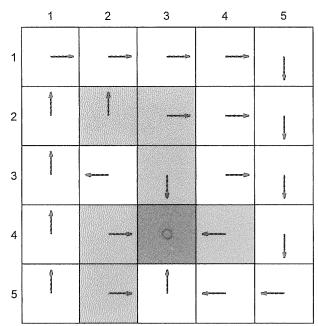
\includegraphics[width=0.32\linewidth]{figures/rl/958edf070871c506f4e013db0a2ac9af4211d7f24f6ec1743cc24414d2cfa0f9}
\end{minipage}

\medskip
{\footnotesize (a) 两个“好”的策略及其对应的状态值。这两个策略的状态值相同，但是它们在第四列的前两个状态是不同的。}

\medskip
% (b) 两个“不好”的策略
\begin{minipage}{\linewidth}
\centering
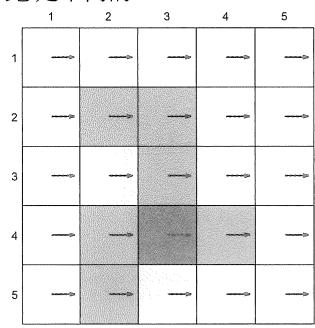
\includegraphics[width=0.22\linewidth]{figures/rl/1f55439a559adfadf1bc4dc891ce4bd3145587b0ddb78bae917ceae536c38b53}\hfill
\begin{minipage}{0.24\linewidth}\centering\footnotesize
\begin{tabular}{c|ccccc}
 & 1 & 2 & 3 & 4 & 5 \\ \hline
1 & $-6.6$ & $-7.3$ & $-8.1$ & $-9.0$ & $-10.0$ \\
2 & $-8.5$ & $-8.3$ & $-8.1$ & $-9.0$ & $-10.0$ \\
3 & $-7.5$ & $-8.3$ & $-8.1$ & $-9.0$ & $-10.0$ \\
4 & $-7.5$ & $-7.2$ & $-9.1$ & $-9.0$ & $-10.0$ \\
5 & $-7.6$ & $-7.3$ & $-8.1$ & $-9.0$ & $-10.0$ \\
\end{tabular}
\end{minipage}\hfill
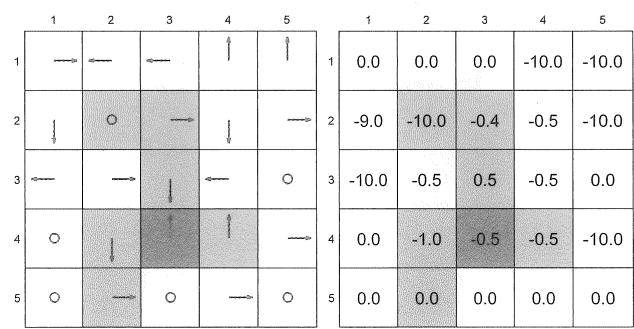
\includegraphics[width=0.22\linewidth]{figures/rl/e9dc1cf5fd4496b6e2b3e398ace38abf32f9a1ca5dc553fba4b9ca27f8bfd4fc}\hfill
\begin{minipage}{0.24\linewidth}\centering\footnotesize
\begin{tabular}{c|ccccc}
 & 1 & 2 & 3 & 4 & 5 \\ \hline
1 & $0.0$ & $0.0$ & $0.0$ & $-10.0$ & $-10.0$ \\
2 & $-9.0$ & $-10.0$ & $-0.4$ & $-0.5$ & $-10.0$ \\
3 & $-10.0$ & $-0.5$ & $0.5$ & $-0.5$ & $0.0$ \\
4 & $0.0$ & $-1.0$ & $-0.5$ & $-0.5$ & $-10.0$ \\
5 & $0.0$ & $0.0$ & $0.0$ & $0.0$ & $0.0$ \\
\end{tabular}
\end{minipage}
\end{minipage}

\medskip
{\footnotesize (b) 两个“不好”的策略及其对应的状态值。这两个策略的状态值比上面两个“好”策略的状态值要小。}
\caption{策略及其对应的状态值的示例。}
\label{fig:rl-bellman-policy-grid}
\end{figure}

% ════════════════════════════════════════════════════════════════
\section{动作值}
\label{sec:rl-bellman-action-value}

到目前为止，本章一直在讨论状态值。下面我们转向动作值或称动作价值（action value）。动作值这个概念非常重要，但之所以在本章的最后一节才介绍它，是因为它依赖于状态值的概念：我们要首先很好地理解状态值，才能很好地理解动作值。

针对一个状态-动作配对（state-action pair）$(s, a)$，其动作值定义为
\begin{equation}
q_\pi(s, a) \doteq \mathbb{E}[G_t \mid S_t = s, A_t = a].
\label{eq:rl-bellman-action-value-def}
\end{equation}
上式表明动作值被定义为在一个状态采取一个动作之后获得的回报的期望值。值得指出的是，$q_\pi(s, a)$ 依赖于一个状态-动作配对 $(s, a)$，而不仅仅是一个动作。因此，或许称这个值为状态-动作值会更严谨，但简便起见，通常称之为动作值。

动作值与状态值有什么关系呢？

\medskip
$\diamond$ 首先，根据条件期望的性质可得
\begin{equation*}
\underbrace{\mathbb{E}[G_t \mid S_t = s]}_{v_\pi(s)} = \sum_{a \in \mathcal{A}} \underbrace{\mathbb{E}[G_t \mid S_t = s, A_t = a]}_{q_\pi(s, a)} \pi(a \mid s).
\end{equation*}
上式可简化为
\begin{equation}
\begin{aligned}
v_\pi(s) &= \sum_{a \in \mathcal{A}} \pi(a \mid s) \, q_\pi(s, a) \\
&= \mathbb{E}_{A_t \sim \pi(s)} \big[ q_\pi(s, A_t) \big].
\end{aligned}
\label{eq:rl-bellman-v-from-q}
\end{equation}
由上式可以看出，状态值是该状态对应的动作值的期望值。

\medskip
$\diamond$ 第二，因为状态值具有如下表达式
\begin{equation*}
v_\pi(s) = \sum_{a \in \mathcal{A}} \pi(a \mid s) \left[ \sum_{r \in \mathcal{R}} p(r \mid s, a) \, r + \gamma \sum_{s' \in \mathcal{S}} p(s' \mid s, a) \, v_\pi(s') \right].
\end{equation*}
将其与 \cref{eq:rl-bellman-v-from-q} 进行比较，可得
\begin{equation}
\begin{aligned}
q_\pi(s, a) &= \sum_{r \in \mathcal{R}} p(r \mid s, a) \, r + \gamma \sum_{s' \in \mathcal{S}} p(s' \mid s, a) \, v_\pi(s') \\
&= \mathbb{E}\big[ R_{t+1} + \gamma v_\pi(S_{t+1}) \mid S_t = s, A_t = a \big].
\end{aligned}
\label{eq:rl-bellman-q-from-v}
\end{equation}
由上式可以看出，动作值是一个包含状态值的变量的期望值。

式 \cref{eq:rl-bellman-v-from-q} 和式 \cref{eq:rl-bellman-q-from-v} 是“一个硬币的两个面”：式 \cref{eq:rl-bellman-v-from-q} 展示了如何从动作值获得状态值，而式 \cref{eq:rl-bellman-q-from-v} 展示了如何从状态值获得动作值。

\subsection{示例}
\label{sec:rl-bellman-action-value-example}

\begin{figure}[H]
\centering
\begin{tikzpicture}[>=Stealth, scale=1.0,
  cell/.style={draw, minimum size=14mm, inner sep=0pt},
  forb/.style={cell, fill=second!22},
  targ/.style={cell, fill=third!20},
  arr/.style={->, thick, main!70!black}]
\node[cell] (s1) at (0,1.4) {$s_1$};
\node[forb] (s2) at (1.4,1.4) {};
\node at (s2) {$s_2$};
\node[cell] (s3) at (0,0) {$s_3$};
\node[targ] (s4) at (1.4,0) {$s_4$};
\node at (s4) {$s_4$};
\node[font=\footnotesize, align=left] at (-0.05,2.25) {$p=0.5$\\ $r=-1$};
\node[font=\footnotesize, align=left] at (-0.6,0.55) {$r=0$\\ $p=0.5$};
\draw[arr] (s1.south) -- (s3.north);
\draw[arr] (s1.east) -- (s2.west);
\draw[arr] (s2.south) -- node[right, font=\footnotesize] {$r=1$} (s4.north);
\draw[arr] (s3.east) -- node[below, font=\footnotesize] {$r=1$} (s4.west);
\node[font=\footnotesize] at (2.1,-0.5) {$r=1$};
\end{tikzpicture}
\caption{用于展示动作值的示例。}
\label{fig:rl-bellman-action-value-example}
\end{figure}

接下来，我们通过一个例子展示如何计算动作值，并特别指出一个初学者常犯的错误。

考虑 \cref{fig:rl-bellman-action-value-example} 中的随机策略。我们下面仅考察状态 $s_1$ 对应的动作值，其他状态是类似的。策略在 $s_1$ 可能会采取两个动作 $a_2$ 或者 $a_3$。首先，$(s_1, a_2)$ 的动作值为
\begin{equation*}
q_\pi(s_1, a_2) = -1 + \gamma v_\pi(s_2),
\end{equation*}
其中 $s_2$ 是下一个状态。类似地，$(s_1, a_3)$ 的动作值是
\begin{equation*}
q_\pi(s_1, a_3) = 0 + \gamma v_\pi(s_3).
\end{equation*}

关于动作值，初学者常犯的一个错误是：因为 \cref{fig:rl-bellman-action-value-example} 中的策略在 $s_1$ 会选择 $a_2$ 或者 $a_3$，而并不会选择 $a_1, a_4, a_5$，所以我们不需要计算 $a_1, a_4, a_5$ 的动作值，或者它们的动作值是 $0$。这是错误的！

\medskip
$\diamond$ 首先，即使一个动作不会被策略选择，它依然具有动作值。在这个例子中，尽管策略 $\pi$ 在 $s_1$ 不会选取 $a_1$，我们仍然可以计算“假如”采取这一动作后将获得的回报。具体来说，在 $s_1$ 选取 $a_1$ 后，智能体会被弹回 $s_1$（因此立即奖励是 $-1$），然后从 $s_1$ 开始按照 $\pi$ 移动（因此未来奖励是 $\gamma v_\pi(s_1)$）。综上，$(s_1, a_1)$ 的动作值为
\begin{equation*}
q_\pi(s_1, a_1) = -1 + \gamma v_\pi(s_1).
\end{equation*}
类似地，对于 $a_4$ 和 $a_5$ 有
\begin{equation*}
\begin{aligned}
q_\pi(s_1, a_4) &= -1 + \gamma v_\pi(s_1), \\
q_\pi(s_1, a_5) &= 0 + \gamma v_\pi(s_1).
\end{aligned}
\end{equation*}

\medskip
$\diamond$ 第二，为什么我们要关心策略不会选择的动作？尽管有些动作可能不会被策略选择，这并不意味着这些动作就不好。相反，这个动作可能是最好的动作，只是因当前的策略不够好而没有选择这个动作罢了。强化学习的目的是寻找最优策略，因此我们必须探索所有动作，从而找到每个状态下的最优动作。

\subsection{基于动作值的贝尔曼方程}
\label{sec:rl-bellman-action-value-bellman}

我们之前介绍的贝尔曼方程都是基于状态值的。实际上，贝尔曼方程也可以用动作值来表达，只是该形式并不常见。不感兴趣的读者可以跳过本节，这并不影响后续的学习。

具体来说，将式 \cref{eq:rl-bellman-v-from-q} 代入式 \cref{eq:rl-bellman-q-from-v} 可以得到
\begin{equation*}
q_\pi(s, a) = \sum_{r \in \mathcal{R}} p(r \mid s, a) \, r + \gamma \sum_{s' \in \mathcal{S}} p(s' \mid s, a) \sum_{a' \in \mathcal{A}(s')} \pi(a' \mid s') \, q_\pi(s', a').
\end{equation*}
这也是一个贝尔曼方程，只不过它只包含动作值而没有状态值。这个方程对每一个状态-动作配对都是成立的。如果我们将所有这些方程都放在一起，则可以得到它们的矩阵-向量形式：
\begin{equation}
q_\pi = \tilde{r} + \gamma P \Pi q_\pi,
\label{eq:rl-bellman-action-mv}
\end{equation}
其中 $q_\pi$ 是一个动作值向量，它对应 $(s, a)$ 的元素是 $[q_\pi]_{(s,a)} = q_\pi(s, a)$；$\tilde{r}$ 是由 $(s, a)$ 索引的即时奖励向量 $[\tilde{r}]_{(s,a)} = \sum_{r \in \mathcal{R}} p(r \mid s, a) \, r$；矩阵 $P$ 是概率转移矩阵，其每一行对应一个状态-动作配对，每一列对应一个状态 $[P]_{(s,a),s'} = p(s' \mid s, a)$；$\Pi$ 是一个块对角矩阵（block diagonal matrix），其中每个块是一个 $1 \times |\mathcal{A}|$ 维的向量：$\Pi_{s',(s',a')} = \pi(a' \mid s')$，而 $\Pi$ 的其他元素都为 $0$。

相比基于状态值的贝尔曼方程，基于动作值的贝尔曼方程具有一些独特的性质。例如，$\tilde{r}$ 和 $P$ 不依赖于策略，仅由系统模型确定，而策略仅被包含在 $\Pi$ 中。更多性质可以参见文献 [5]。

% ════════════════════════════════════════════════════════════════
\section{总结}
\label{sec:rl-bellman-summary}

本章介绍的最重要的概念是状态值。数学上，状态值是智能体从一个状态出发所能获得的回报的期望值。

不同状态的值是彼此相关的。例如，状态 $s$ 的值依赖于一些其他状态的值，而其他这些状态的值可能又依赖于更多其他状态或者状态 $s$ 的值。这种关系可能是对初学者来说最困惑的一点，它涉及一个自举的重要概念。“自举”的英文翻译是 bootstrapping，它在不同历史时期有不同的含义。从字面上来讲，它指的是鞋后边能够帮助更好地穿鞋的带子，后来它用于讽刺那些异想天开的想法，如自己想通过双手拉着自己鞋上的两个带子让自己的双脚离地；它的现代引申意义指的是自迭代算法，即从一个初始值出发不断迭代计算。

虽然从直觉上来看自举是比较令人困惑的，但是从数学上来看，贝尔曼方程清晰地描述了不同状态值之间的关系，以及如何通过迭代的方式求解状态值。此外，由于状态值可用于评价策略的优劣，因此根据贝尔曼方程求解某一策略的状态值的过程称为策略评价。正如本书后面介绍的，策略评价是强化学习算法中的重要步骤。

本章介绍的另一个重要概念是动作值，它可以描述在某个状态采取某个动作的价值。正如本书后面会介绍的，当我们尝试寻找最优策略时，动作值相比状态值将发挥更直接的作用。

最后，贝尔曼方程并不局限于强化学习领域，它在许多领域如控制理论和运筹学中都有广泛应用。在不同领域，贝尔曼方程可能有不同的表达形式。本书是在离散马尔可夫决策过程的框架下介绍贝尔曼方程的，更多的信息可以参见文献 [2]。

% ════════════════════════════════════════════════════════════════
\section{问答}
\label{sec:rl-bellman-qa}

\medskip
$\diamond$ \textbf{提问}：状态值和回报之间的关系是什么？

\textbf{回答}：一个状态的状态值是智能体从该状态出发可以获得的回报的期望值。

\medskip
$\diamond$ \textbf{提问}：我们为什么要关心状态值？它为什么重要？

\textbf{回答}：状态值可以用来评价策略的好坏。在下一章我们将看到，最优策略就是基于状态值来定义的。

\medskip
$\diamond$ \textbf{提问}：我们为什么要关心贝尔曼方程？它为什么重要？

\textbf{回答}：贝尔曼方程描述了所有状态值之间的关系，它是分析和求解状态值的核心工具。

\medskip
$\diamond$ \textbf{提问}：为什么求解贝尔曼方程的过程被称为策略评价？

\textbf{回答}：求解贝尔曼方程得到的是状态值，由于状态值可以用来评价策略，因此求解贝尔曼方程的过程可以被理解为评价相应的策略。

\medskip
$\diamond$ \textbf{提问}：我们为什么需要研究贝尔曼方程的矩阵-向量形式？

\textbf{回答}：贝尔曼方程是为所有状态建立的一组线性方程。为了求解所有状态值，我们有必要联立这些方程，而其矩阵-向量形式则是这些方程联立之后的简洁表达式。

\medskip
$\diamond$ \textbf{提问}：状态值与动作值之间的关系是什么？

\textbf{回答}：它们的关系可以通过式 \cref{eq:rl-bellman-v-from-q} 和式 \cref{eq:rl-bellman-q-from-v} 清晰地阐述，它们相互依赖，可以相互转换。

\medskip
$\diamond$ \textbf{提问}：我们为什么关心一个给定策略不会选择的动作的价值？

\textbf{回答}：尽管一个给定的策略可能不会选择某些动作，但是这并不意味着这些动作是不好的。相反，有可能是因给定的策略不够好而错过了最好的动作。因此，为了寻找更好的策略，我们要探索所有动作，即使其中一些可能不会被当前给定策略选择，这一点在后面介绍基于蒙特卡罗的强化学习算法时会更加明显，读者现在只需要有一个大概的理解即可。
